% !TeX encoding = UTF-8
% !TeX spellcheck = de_DE
% !TeX program = lualatex
% !TeX BIB program = biber
%other magic comments: see TeXstudio user manual, chapter 4.10
\documentclass{standalone}

\usepackage{tikz}
\usetikzlibrary{circuits.ee.IEC}

\title{Dreiwegeweiche}
\author{Wolfgang~Witt}
\date{\today}

\begin{document}
	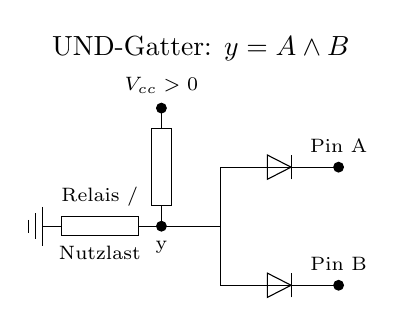
\begin{tikzpicture}[circuit ee IEC, every info/.style={font=\scriptsize}]
		\draw node (vcc) [contact, info={$V_{cc}>0$}] {} to[resistor] ++(0,-1.5) node (contact) [contact, info'={y}] {} to ++(.75,0) node (splitAB) {} to ++(0,.75) to [diode] ++(1.5,0) node (PinA) [contact, info={Pin A}] {};
		\draw (splitAB.center) to ++(0,-.75) to [diode] ++(1.5,0) node (PinB) [contact, info={Pin B}] {};
		\draw (contact) to [resistor={info'={Relais /}, info={Nutzlast}}] ++(-1.5,0) node (ground) [ground, anchor=west, rotate=180] {};
		%Überschrift
		\path (vcc) ++(.5, .75) node {UND-Gatter: $y = A \wedge B$};
	\end{tikzpicture}
\end{document}
